\documentclass[12pt]{article}
\usepackage{fullpage}
\usepackage{graphicx}
\newtheorem{definition}{Definition}
\newtheorem{question}{Question}
\newtheorem{property}{Property}
\newtheorem{proof}{\em Proof}
\newtheorem{derivation}{\em Sketch}
\newtheorem{notation}{Notation}

\newcommand{\comment}[1]{}
\newcommand{\VS}{\mbox{\it VS}}
\newcommand{\WM}{\mbox{\it WM}}
\newcommand{\PCONJ}{\mbox{\it PCONJ}}
\newcommand{\kDNF}{\mbox{\it kDNF}}
\newcommand{\PDISJ}{\mbox{\it PDISJ}}
\newcommand{\DTrt}{\mbox{\it DT}_{r2}}
\newcommand{\DTs}{\mbox{\it DT}_s}
\newcommand{\PP}{{\rm P}}
\newcommand{\EE}{{\rm E}}
\newcommand{\PX}{\PP_{\!\scriptscriptstyle\! X}}
\newcommand{\PXY}{\PP_{\!\scriptscriptstyle\! X\!Y}}
\newcommand{\PYX}{\PP_{\!\scriptscriptstyle\! Y\!|\!X}}
\newcommand{\PYx}{\PP_{\!\scriptscriptstyle\! Y\!|x}}
\newcommand{\seq}[1]{\langle{#1}\rangle}
\newcommand{\RR}{I\!\!R}
\newcommand{\NN}{I\!\!N}
\newcommand{\argmin}{\arg\!\min}
\newcommand{\argmax}{\arg\!\max}
\newcommand{\eg}{{\em e.g.},\ }
\newcommand{\Eg}{{\em E.g.},\ }
\newcommand{\ie}{{\em i.e.},\ }
\newcommand{\Ie}{{\em I.e.},\ }
\newcommand{\cf}{{\em cf.}\ }
\newcommand{\etc}{{\em etc}}
\newcommand{\aka}{{\em a.k.a.}}
\newcommand{\vardef}{\stackrel{\triangle}{=}}
\def\norm [#1]{{\| #1 \|}}
\newcommand{\sign}{\mbox{\rm sign}}
\newcommand{\err}{\mbox{\rm err}}
\newcommand{\rank}{\mbox{\rm rank}}
\newcommand{\cond}{\mbox{\rm cond}}
\newcommand{\vect}{\mbox{\rm vec}}
\newcommand{\tr}{\mbox{\rm tr}}
\newcommand{\set}[1]{{\{#1\}}}
\newcommand{\tnorm}[2]{\|{#1}\|_{#2}}
\newcommand{\normdot}{{\mbox{$\|\!\cdot\!\|$}}}

%\newcommand{\makevector}[1]{{\tilde{#1}}}
\newcommand{\makevector}[1]{{\bf #1}}
\newcommand{\fvec}{{\makevector{f}}}
\newcommand{\evec}{{\makevector{e}}}
\newcommand{\bvec}{{\makevector{b}}}
\newcommand{\rvec}{{\makevector{r}}}
\newcommand{\dvec}{{\makevector{d}}}
\newcommand{\xvec}{{\makevector{x}}}
\newcommand{\qvec}{{\makevector{q}}}
\newcommand{\yvec}{{\makevector{y}}}
\newcommand{\mvec}{{\makevector{m}}}
\newcommand{\vvec}{{\makevector{v}}}
\newcommand{\zvec}{{\makevector{z}}}
\newcommand{\avec}{{\makevector{a}}}
\newcommand{\wvec}{{\makevector{w}}}
\newcommand{\cvec}{{\makevector{c}}}
\newcommand{\Xvec}{{\makevector{X}}}
\newcommand{\Fvec}{{\makevector{F}}}
\newcommand{\Avec}{{\makevector{A}}}
\newcommand{\Bvec}{{\makevector{B}}}
\newcommand{\Hvec}{{\makevector{H}}}
\newcommand{\Lvec}{{\makevector{L}}}
\newcommand{\Mvec}{{\makevector{M}}}
\newcommand{\Nvec}{{\makevector{N}}}
\newcommand{\Vvec}{{\makevector{V}}}
\newcommand{\Uvec}{{\makevector{U}}}
\newcommand{\Ivec}{{\makevector{I}}}
\newcommand{\Ovec}{{\makevector{O}}}
\newcommand{\smallxvec}{{\scriptsize\mathbf x}}
\newcommand{\alphavec}{\mbox{\boldmath $\alpha$}}
\newcommand{\betavec}{\mbox{\boldmath $\beta$}}
\newcommand{\muvec}{\mbox{\boldmath $\mu$}}
\newcommand{\phivec}{{\mbox{\boldmath $\phi$}}}
\newcommand{\lambdavec}{\mbox{\boldmath $\lambda$}}
\newcommand{\Lambdavec}{\mbox{\boldmath $\Lambda$}}
\newcommand{\Sigmavec}{\mbox{\boldmath $\Sigma$}}
\newcommand{\yy}{{\tt y}}
\newcommand{\uu}{{\tt u}}
\newcommand{\zerovec}{{\makevector{0}}}
\newcommand{\smallzerovec}{{\scriptsize\bf 0}}
\newcommand{\smallonevec}{{\scriptsize\bf 1}}
\newcommand{\onevec}{{\makevector{1}}}
\newcommand{\smallbetavec}{\mbox{\scriptsize\boldmath $\beta$}}
\newcommand{\smallmuvec}{\mbox{\scriptsize\boldmath $\mu$}}


\begin{document}

\noindent
{\Large\bf AUCSC 460 -- Artificial Intelligence}

\vspace*{1\baselineskip}

\noindent
{\large\bf Assignment 1: Knowledge Representation and Reasoning}

\vspace*{1\baselineskip}

\noindent
Winter 2016\\
Department of Science\\
University of Alberta, Augustana Faculty

\vspace*{1.75\baselineskip}
\hrule

\vspace*{0.75\baselineskip}

\noindent
{\bf Due}: through eClass, {\em Monday, January 25}\\
{\bf Worth}: 25\% of final grade
\\
{\bf Instructor}: Anna Koop, HB 1-31, akoop@ualberta.ca

\vspace*{0.75\baselineskip}

\hrule

\vspace*{1\baselineskip}

\noindent
{\bf Note}
Please submit your assignment to me by email.
Some of the questions require you to write small programs,
however for the written questions please format your answers
in a single {\em pdf} file.
Submit all required documents in a zip or tar archive.


\vspace*{1\baselineskip}

\hrule

\section*{Part 1: Propositional Logic}
Reference: Ch 7 of AIMA, Lectures 3-4.

%%%%%%%%%%%%
\subsection*{Question 1 \rm(Circuit Representation in Propositional Logic---2\%)}
Digital logic circuits map easily onto propositional logic, meaning that reasoning about propositional logic has direct practical application in computer design.
\begin{center}
\begin{tabular}[h]{r | l}
Circuit Design & Propositional Logic \\
\hline
circuit & complex sentence\\
logic gate & connective \\
input wire & atomic sentence \\
voltage & truth value
\end{tabular}
\end{center}

Write out the formula for the circuit below (Figure \ref{fig:adder}) and convert it to conjunctive normal form. Show your steps.
\begin{figure}[bt]
\caption{A (claimed) full-adder circuit}
\label{fig:adder}
\centering
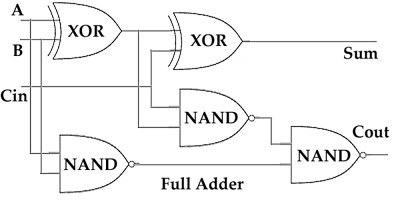
\includegraphics[width=.6\textwidth]{full_adder.png}
\end{figure}


%%%%%%%%%%%%
\subsection*{Question 2 \rm(Applied Satisfiability---3\%)}
A digital circuit that only ever returns 0 is not going to be a terribly useful addition to a circuit board. Describe an algorithm (in words, pseudocode, or your language of choice) that, given a sentence in propositional logic, returns T if there exists an input configuration that results in non-zero output and F if there is no possible input that results in non-zero output.

%%%%%%%%%%%%
\subsection*{Question 3 \rm(Proving equivalence---5\%)}
It is not uncommon for perfectly functional circuits to be redesigned (eg. in order to save energy or materials or to fit more compactly on the board). An important step before manufacturing is to verify that the new design is equivalent to the old. Describe an algorithm that will take the logical formula for both circuits and return T if they are equivalent and F if they are not.

%%%%%%%%%%%%
\section*{Part 2: Knowledge Engineering}
Reference: Ch 8 of AIMA, Lectures 5-6.

You will be designing an expert system for validating circuit designs. You may use whatever language, libraries or references you like, but you must be able to explain clearly how they work. I suggest using the Knowledge Base code supplied on the textbook website, which we discussed in lab. You will need to submit your working KB code as well as sufficient documentation for populating it.

%%%%%%%%%%%%
\subsection*{Question 4 \rm(Ontology---2\%)}
What concepts do you need in this expert system? Describe the predicate symbols, functions, and constants you will be using. 

%%%%%%%%%%%%
\subsection*{Question 5 \rm(Axioms---4\%)}
What general rules must this expert system use to understand systems? These should be universal, separate from the KB augmented for a specific circuit design.

Submit a populated knowledge base for this question (either the saved state or code for populating it).

\subsection*{Question 6 \rm(Querying--8\%)}
Use your knowledge base to determine whether the circuit below (Figure \ref{fig:sat}) is satisfiable. Note to do so you must populated the KB with the information about the specific circuit and formulate the satisfiability question as a logical query. Submit the updated knowledge base and the query itself, as well as the answer.

\begin{figure}[bt]
\caption{An unknown circuit}
\label{fig:sat}
\centering
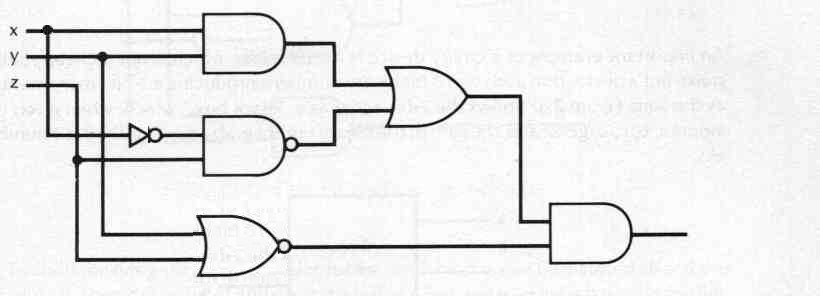
\includegraphics[width=.8\textwidth]{circuit2.jpg}
\end{figure}



\end{document}
